\documentclass{article}
\linespread{1.3}
\usepackage[margin=50pt]{geometry}
\usepackage{amsmath, amsthm, amssymb, amsthm, tikz, fancyhdr, graphicx, systeme}
\pagestyle{fancy}
\renewcommand{\headrulewidth}{0pt}
\newcommand{\changefont}{\fontsize{15}{15}\selectfont}

\fancypagestyle{firstpageheader}{
  \fancyhead[R]{
    \changefont
    \parbox[t]{4cm}{ % Adjust width as needed
      Michael Huang\\
      EN.625.603.84\\
      Problem Set \#6
    }
  }
}

\begin{document}

\thispagestyle{firstpageheader}
{\Large 

\section*{6.2.8b}
Calculate the P-values for the hypothesis tests indicated in Question 6.2.1. Do they agree with your decisions on whether or not to reject \(H_0\)?
\\
\\
With the inequality, we know that this is a two-tailed test. We therefore calculate the test statistic as 
\[
\frac{\bar{y} - \mu_0}{\sigma / \sqrt{n}} = \frac{45.1 - 42.9}{3.2 / \sqrt{16}} = \frac{2.2}{3.2 / 4} = 2.75
\]
Using a table, we can also determine the critical z-value \(z_{\alpha / 2} = z_{0.01 / 2} = z_{0.005} = \) approximately -2.58 with corresponding value 0.00494. The absolute value of the test statistic is greater than the absolute value of the critical z-value, so we reject \(H_0\). Now, looking at the p-value, using a z-table we find the corresponding value for 2.75 to be 0.00298, and we multiply by 2 for both tails to find this to be \(2 \cdot 0.00298 = 0.00596\), which is smaller than the given \(\alpha = 0.01\), which indicates that we should also reject \(H_0\). This does indeed agree with the previously determined decision to reject \(H_0\).

\section*{6.3.7}
What \(\alpha\) levels are possible with a decision rule of the form “Reject \(H_0\) if \(k \geq k*\)” when \(H_0: p = 0.5\) is to be tested against \(H_1: p > 0.5\) using a random sample of size \(n = 7\)?
\\
\\
As this is a decision with two distinct choices, we can take the binomial with \(n = 7\) to find the probabilities \(\binom{7}{k} \cdot 0.5^7\):
\begin{equation*}
\begin{cases}
P(k = 0) = \binom{7}{0} \cdot \frac{1}{2}^7 = \frac{7!}{0!7!} \cdot \frac{1}{2}^7 = \frac{1}{128} \\ 
P(k = 1) = \binom{7}{1} \cdot \frac{1}{2}^7 = \frac{7!}{1!6!} \cdot \frac{1}{2}^7 = \frac{7}{128} \\ 
P(k = 2) = \binom{7}{2} \cdot \frac{1}{2}^7 = \frac{7!}{2!5!} \cdot \frac{1}{2}^7 = \frac{42}{2 \cdot 128} = \frac{21}{128} \\ 
P(k = 3) = \binom{7}{3} \cdot \frac{1}{2}^7 = \frac{7!}{3!4!} \cdot \frac{1}{2}^7 = \frac{210}{6 \cdot 128} = \frac{35}{128} \\ 
P(k = 4) = \binom{7}{4} \cdot \frac{1}{2}^7 = \frac{7!}{3!4!} \cdot \frac{1}{2}^7 = \frac{35}{128} \\ 
P(k = 5) = \binom{7}{5} \cdot \frac{1}{2}^7 = \frac{7!}{2!5!} \cdot \frac{1}{2}^7 = \frac{21}{128} \\ 
P(k = 6) = \binom{7}{6} \cdot \frac{1}{2}^7 = \frac{7!}{1!6!} \cdot \frac{1}{2}^7 = \frac{7}{128} \\ 
P(k = 7) = \binom{7}{7} \cdot \frac{1}{2}^7 = \frac{7!}{0!7!} \cdot \frac{1}{2}^7 = \frac{1}{128} \\ 
\end{cases}
\end{equation*}
We can then determine \(\alpha = P(k \geq k* | H_0) = P(k \geq k* | p = 0.5) = 1 - P(k < k)\) for each possible value: 
\begin{equation*}
\begin{cases}
\alpha_{k* = 0} = P(k \geq 0) = 1 - 0 = 1 \\
\alpha_{k* = 1} = P(k \geq 1) = 1 - \frac{1}{128} = \frac{127}{128} \\
\alpha_{k* = 2} = P(k \geq 2) = 1 - \frac{1 + 7}{128} = \frac{120}{128} = \frac{15}{16} \\
\alpha_{k* = 3} = P(k \geq 3) = 1 - \frac{1 + 7 + 21}{128} = \frac{99}{128} \\
\alpha_{k* = 4} = P(k \geq 4) = 1 - \frac{1 + 7 + 21 + 35}{128} = \frac{64}{128} = \frac{1}{2} \\
\alpha_{k* = 5} = P(k \geq 5) = 1 - \frac{1 + 7 + 21 + 35 + 35}{128} = \frac{29}{128} \\
\alpha_{k* = 6} = P(k \geq 6) = 1 - \frac{1 + 7 + 21 + 35 + 35 + 21}{128} = \frac{8}{128} = \frac{1}{16} \\
\alpha_{k* = 7} = P(k \geq 7) = \frac{1}{128} \\
\alpha_{k* = 8, \text{etc.}} = P(k \geq 8) = 0 \\
\end{cases}
\end{equation*}

\section*{6.4.3}
For the decision rule found in Question 6.2.2 to test \(H_0: \mu = 95\) versus \(H_1:\mu \neq 95\) at the \(\alpha = 0.06\) level of significance, calculate \(1 - \beta\) when \(\mu = 90\).
\\
\\
This requires a two-tailed setup to account for \(\mu < 95\) and \(\mu > 95\). We can standardize with the given \(n=22\), standard deviation \(\sigma = 15\), and z-value corresponding to \(\frac{0.06}{2} = 0.03\) (due to the two-tailed nature) which is about 1.88 at 0.03005, we can demonstrate this to be 
\[
\frac{\bar{Y} - \mu_0}{\sigma/\sqrt{n}} < -1.88
\]
\[
\frac{\bar{Y} - 95}{15 / \sqrt{22}} < -1.88
\]
\[
\bar{Y} < 95 + -1.88 \cdot \frac{15}{\sqrt{22}} = 88.9877397988
\]
and 
\[
\frac{\bar{Y} - \mu_0}{\sigma/\sqrt{n}} > 1.88
\]
\[
\frac{\bar{Y} - 95}{15 / \sqrt{22}} > 1.88
\]
\[
\bar{Y} > 95 + 1.88 \cdot \frac{15}{\sqrt{22}} = 101.012260201
\]
So in the context of the power calculation, we have \(1 - \beta = P(\text{Reject }H_0 | H_1 \text{ is true}) = P(\bar{Y} < 88.9877397988 \text{ or } \bar{Y} > 101.012260201 | \mu = 90) \) which translates to 
\[
1 - \beta = P(\frac{\bar{Y} - 90}{15 / \sqrt{22}} < \frac{88.9877397988 - 90}{15 / \sqrt{22}}) + P(\frac{\bar{Y} - 90}{15 / \sqrt{22}} > \frac{101.012260201 - 90}{15 / \sqrt{22}})
\]
\[
= P(Z < \frac{-1.0122602012}{3.19801074533}) + P(Z > \frac{11.012260201}{3.19801074533})
\]
\[
= P(Z < -0.31652808005) + P(Z > 3.44347191987)
\]
\[
= 0.37448 + (1 - 0.99971) = 0.37448 + 0.00029 = 0.37477
\]

\section*{6.4.4}

Construct a power curve for the \(\alpha = 0.05\) test of \(H_0: \mu = 60\) versus \(H_1: \mu \neq 60\) if the data consist of a random sample of size 16 from a normal distribution having \(\sigma = 4\).
\\
\\
To construct the power curve, we need to first find the critical values for two-tailed test. As the standard deviation is known to be \(\sigma = 4\), we need to find z-value \(\frac{\bar{x} - \mu_0}{\sigma / \sqrt{n}} = \frac{\bar{x} - 60}{4 / \sqrt{16}} = \bar{x} - 60\). We can find the critical values to be \(z_{\alpha / 2} = z_{0.05 / 2} = z_{0.025} = -1.9599639845400545\), so essentially +/-1.9599639845400545 due to the nature of the two-tailed test. To know how to determine the cdf, to be plotted, we can now adjust using the standard error \(\frac{\sigma}{\sqrt{n}} = \frac{4}{\sqrt{16}} = 1\). We therefore just need to take the cdfs of the ranges \(\bar{x} < 60 - 1.9599639845400545 \cdot 1 = 58.0400360155\) and \(\bar{x} > 60 + 1.9599639845400545 \cdot 1 = 61.9599639845\). We can therefore plot the power as a function of the means \(\mu\):
\[
P(z < 58.0400360155) + P(z > 61.9599639845)
\]
\[
cdf(58.0400360155 - \mu) + 1 - cdf(61.9599639845 - \mu)
\]
\\
\\ 
Based off these values, I wrote a script in Python to generate the following power curve:
\begin{figure}[h!]
  \centering
  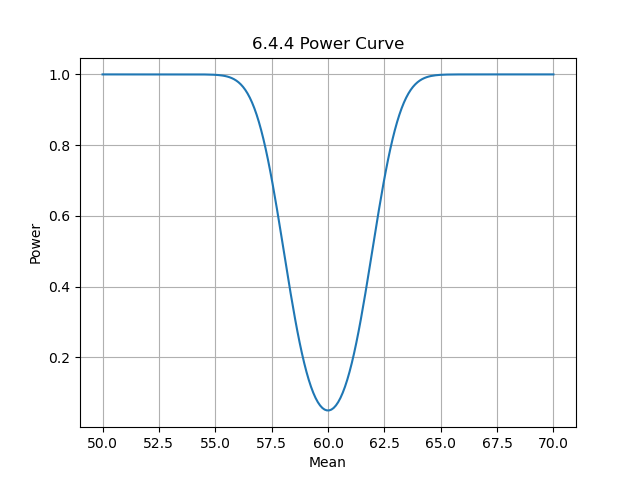
\includegraphics[width=500pt]{power_curve.png}
\end{figure}
\\
\\
\\ \\ \\ \\ \\ \\ \\ \\ \\ \\ \\ \\ \\ \\
The code I used is as follows:
\begin{verbatim}
import numpy as np
import matplotlib.pyplot as plt
from scipy import stats

curve_z_value = stats.norm.ppf(0.05 / 2)

print(f"{curve_z_value=}")

mean_values = np.linspace(50, 70, 200)
beta_values = stats.norm.cdf(58.04 - mean_values) + (1 - stats.norm.cdf(61.96 - mean_values))

plt.plot(mean_values, beta_values)
plt.xlabel("Mean")
plt.ylabel("Power")
plt.title("6.4.4 Power Curve")
plt.grid(True)
plt.show()
\end{verbatim}

\section*{6.4.7} 

If \(H_0: \mu = 200\) is to be tested against \(H_1: \mu < 200\) at the \( \alpha = 0.10\) level of significance based on a random sample of size \(n\) from a normal distribution where \(\sigma = 15.0\), what is the smallest value for \(n\) that will make the power equal to at least 0.75 when \(\mu = 197\)?
\\
\\
This is a left-tailed test. We first find the corresponding critical value, finding the z-value using a table corresponding to \(\alpha = 0.10\) to be about -1.28 with value 0.10027. We then use this relative to the given sample mean to get the corresponding \(\bar{Y}\):
\[
\frac{\bar{Y} - \mu_0}{\sigma / \sqrt{n}} < -1.28
\]
\[
\frac{\bar{Y} - 200}{15 / \sqrt{n}} < -1.28
\]
\[
\bar{Y} < \frac{-1.28}{15 / \sqrt{n}} + 200
\]
Translating what we've found so far to the desired power condition,  we have
\[
P(\text{reject }H_0 | \mu = 197) = P(\bar{X} < X | \mu = 197) \geq 0.75
\]
\[
P(\bar{X} < \frac{-1.28}{15 / \sqrt{n}} + 200 | \mu = 197) \geq 0.75
\]
and standardizing:
\[
P(\frac{\bar{X} - 197}{15 / \sqrt{n}} < \frac{\frac{-1.28}{15 / \sqrt{n}} + 200 - 197}{15 / \sqrt{n}}) \geq 0.75
\]
\[
P(z < \frac{\frac{-1.28}{15 / \sqrt{n}} + 200 - 197}{15 / \sqrt{n}}) \geq 0.75
\]
\[
P(z < -1.28 + \frac{\sqrt{n}}{5}) \geq 0.75
\]
To solve this, we first find the corresponding z-value for 0.75, looking at a table we find this to be approximately 0.67 with corresponding value 0.74857. We can then continue solving:
\[
-1.28 + \frac{\sqrt{n}}{5} = 0.674
\]
\[
\frac{\sqrt{n}}{5} = 1.954
\]
\[
n = (1.954 \cdot 5)^2 = 95.4529
\]
but as we need a whole number \(n\), we round up to find that \(n = 96\).

\section*{6.4.9}

If \(H_0: \mu = 30\) is tested against \(H_1: \mu > 30\) using \(n = 16\) observations (normally distributed) and if \(1 - \beta = 0.85\) when \(\mu = 34\), what does \(\alpha\) equal? Assume that \(\sigma = 9\).
\\
\\
This is a right-tailed test. Using the normal distribution, we can take the Z-value that we want to not exceed to be \(\frac{\bar{Y} - \mu_0}{\sigma/\sqrt{n}} = \frac{\bar{Y} - 30}{9 / \sqrt{16}} = \frac{\bar{Y} - 30}{9 / 4}\), so we want to find 
\[
\bar{Y} = \frac{9}{4}z + 30
\]
We can interpret from \( 1 - \beta = 0.85 = P(\text{reject } H_0 | \mu = 34) = P(Y > \bar{Y} | \mu = 34)\). We can translate this to be 
\[
P(\frac{\bar{Y} - 34}{9 / 4} > \frac{\frac{9}{4}z + 30 - 34}{9/4}) = 0.85
\]
\[
P(z > \frac{\frac{9}{4}z + 30 - 34}{9/4}) = 0.85
\]
\[
P(z > z - \frac{16}{9}) = 0.85
\]
\[
P(z > z - \frac{16}{9}) = 0.85
\]
We can interpret this as the right tail being 0.85, so the left tail would be 0.15, which looking up in a table we can find the corresponding z value to be approximately -1.04 with corresponding value 0.14917. So we essentially just need to find corresponding value to solve 
\[
z - \frac{16}{9} = -1.04
\]
\[
z = 0.73777777778
\]
We can interpret this in the context of \(\alpha\) as the probability of rejecting \(H_0\) when it holds, i.e. \(P(z > z) = \alpha\) as we will reject when we surpass this given z-value. Taking ~0.74 and looking it up in a table, we get the value to be \(\alpha = 0.77035 \).

\section*{7.3.2}

Find the moment-generating function for a chi square random variable and use it to show that \(E (\chi^2_n) = n \) and \(Var(\chi^2_n) = 2n\).
\\
\\
We previously defined the chi square distribution as \(\sum_{i=1}^{n} Z^2_i\), where the \(Z_i\)'s are independent standard normal random variables. We can find \(M(t)\) by definition as follows, first using the individual components themselves and then taking the product:
\[
M_{Z_i^2}(t) = E(e^{tZ_i^2}) = \int_{-\infty}^{\infty} e^{tz^2} f(z) dz  = \int_{-\infty}^{\infty} e^{tz^2} \cdot \frac{1}{\sqrt{2\pi}}e^{-z^2/2} dz
\]
\[
= \frac{1}{\sqrt{2\pi}}\int_{-\infty}^{\infty} e^{tz^2-z^2/2} dz = \frac{1}{\sqrt{2\pi}}\int_{-\infty}^{\infty} e^{(1-2t) \cdot -z^2/2} dz
\]
integration by substitution, with \(u = z\sqrt{1 - 2t}\), \(du = \sqrt{1 - 2t} dz\), and thus \(dz = \frac{du}{\sqrt{1 - 2t}}\):
\[
= \frac{1}{\sqrt{2\pi}} \int_{-\infty}^{\infty} e^{-u^2 / 2} \cdot \frac{du}{\sqrt{1 - 2t}} = \frac{1}{\sqrt{2\pi}} \frac{1}{\sqrt{1 - 2t}} \int_{-\infty}^{\infty} e^{-u^2 / 2} du
\]
We note this follows the standard normal distribution pdf \(f_x = \frac{1}{\sqrt{2\pi}} e^{-x^2 / 2}\), which is has property \(\int_{-\infty}^{\infty} f_x dx = 1\) and therefore \(\int_{-\infty}^{\infty} e^{-z^2 / 2} dz = \sqrt{2\pi}\):
\[
= \frac{1}{\sqrt{2\pi}} \cdot \frac{1}{\sqrt{1 - 2t}} \cdot \sqrt{2\pi} = \frac{1}{\sqrt{1 - 2t}}
\]
We can now finally find
\[
M_{\chi_n^2} (t) = \prod_{i=1}^{n} M_{\chi_i^2} (t) = (\frac{1}{\sqrt{1 - 2t}})^n = (1-2t)^{-1/2 \cdot n} = (1-2t)^{-n/2}
\]
Now, use this to find \(E(\chi^2_n)\):
\[
E(\chi^2_n) = M'_{\chi_n^2} (0) = \frac{d}{dt} (1-2t)^{-n/2} |_{t=0} = \frac{-n}{2} \cdot (1-2t)^{-n/2 - 1} \cdot -2 |_{t=0}
\]
\[
= \frac{-n}{2} \cdot -2 \cdot (1-2t)^{-n/2 - 1} |_{t=0} = n \cdot (1-2t)^{-n/2 - 1} |_{t=0} = n (1 - 0)^{-n/2 - 1} = n
\]
as we expected. Next, to find \(Var(\chi^2_n)\), we need to determine \(E({\chi_n^2}^2)\):
\[
E({\chi_n^2}^2) = M''_{\chi_n^2} (0) = \frac{d}{dt} [n(1-2t)^{-n/2 - 1}] = (-n/2 - 1) \cdot n \cdot (1-2t)^{-n/2 - 2} \cdot -2 |_{t = 0}
\]
\[
-(n/2 + 1) \cdot n \cdot -2 \cdot (1-2t)^{-n/2 - 2} |_{t = 0} = (n^2 + 2n)(1 - 0)^{-n/2 - 2} = n^2 + 2n
\]
So therefore we have 
\[
Var(\chi_n^2) = E({\chi_n^2}^2) - E(\chi_n^2)^2 = n^2 + 2n - n^2 = 2n
\]
exactly as we hoped to show.

\section*{7.4.5}

Suppose a random sample of size \(n = 11\) is drawn from a normal distribution with \(\mu = 15.0\). For what value of \(k\) is the following true? 
\[
P(\left|\frac{\bar{Y} - 15.0}{S / \sqrt{11}}\right| \geq k) = 0.05
\]
\\
\\
We see that the middle expression follows a t-distribution with \(n = 11\) and therefore \(df = n - 1 = 10\). We can therefore rewrite this expression in the form \(P(|T| \geq k) = 0.05\) for the corresponding distribution \(T\). Since this is two-tailed, we can also determine the corresponding critical values by using \(\alpha = 0.05\), so we would find the corresponding value for \(t_{\alpha / 2, df = n-1} = t_{0.05 / 2, 11 - 1} = t_{0.025, 10}\), which we can determine to be -2.2281388519649385. \(k\) is therefore 2.228138851964938. 
\\
\\
The code used is as follows:
\begin{verbatim}
from scipy import stats

k_t_value = stats.t.ppf(0.05 / 2, 10)

print(f"{k_t_value=}")
\end{verbatim}
with output:
\begin{verbatim}
~/Doc/e/j/S/Problem Sets/EN.625.603.84/Problem Set 6 problem-set-5 ?1 .......................... py base 23:18:57
> python k_value_745.py 
k_t_value=np.float64(-2.2281388519649385)
\end{verbatim}

\section*{7.4.9}

\subsection*{(a)}

What can be inferred from these data about the \(true\) average age at which scientists do their best work? Answer the question by constructing a 95\% confidence interval.
\\
\\
We can take the mean from the 12 ages given, and also do find the mean and sample standard deviation using the standard formula with the sum of squared differences from the mean divided by \(n - 1 = 11\), and then square rooted. We do this in Python to save time. We find the mean to be 35.416666666666664 and the standard deviation to be 7.229464123650627. We can now use the t-distribution for confidence interval to determine the standard error from which we should expect to deviate from the mean for the desired confidence interval. We need to find \(t_{\alpha / 2, df} = t_{(1 - 0.95) / 2, 12 - 1} = t_{0.05 / 2, 11} = t_{0.025, 11}\) which we determine using Python to be -2.200985160082949, so we can find the deviation from the mean to be \(t \cdot \frac{s}{\sqrt{n}} = -2.200985160082949 \cdot \frac{7.229464123650627}{\sqrt{12}} = -2.200985160082949 \cdot 2.08696652894 = -4.59338235979 \). So the true average age would be the mean +/- this difference, so it would be \(35.416666666666664 +/- 4.59338235979\) years, or approximately 30.8 to 40 years old.
\\
\\
The code used is as follows:
\begin{verbatim}
import numpy as np
from scipy import stats

ages = [40, 34, 23, 40, 31, 33, 49, 33, 34, 43, 26, 39]

print(f"{len(ages)=}")

ages_mean = np.mean(ages)
ages_sd = np.std(ages, ddof=1)

print(f"{ages_mean=}")
print(f"{ages_sd=}")

ages_t_value = stats.t.ppf(0.05 / 2, 11)

print(f"{ages_t_value=}")
\end{verbatim}
with output:
\begin{verbatim}
~/Doc/e/j/S/Problem Sets/EN.625.603.84/Problem Set 6 problem-set-5 ?1 .......................... py base 01:45:15
> python science_749.py
len(ages)=12
ages_mean=np.float64(35.416666666666664)
ages_sd=np.float64(7.229464123650627)
ages_t_value=np.float64(-2.200985160082949)
\end{verbatim}

\subsection*{(b)}

Before constructing a confidence interval for a set of observations extending over a long period of time, we should be convinced that the \(y_i\)'s exhibit no biases or trends. If, for example, the age at which scientists made major discoveries decreased from century to century, then the parameter \(\mu\) would no longer be a constant, and the confidence interval would be meaningless. Plot “date” versus “age” for these twelve discoveries. Put “date” on the abscissa. Does the variability in the \(y_i\)'s appear to be random with respect to time?
\\
\\
Let's do some plotting with Python: 
\begin{figure}[h!]
  \centering
  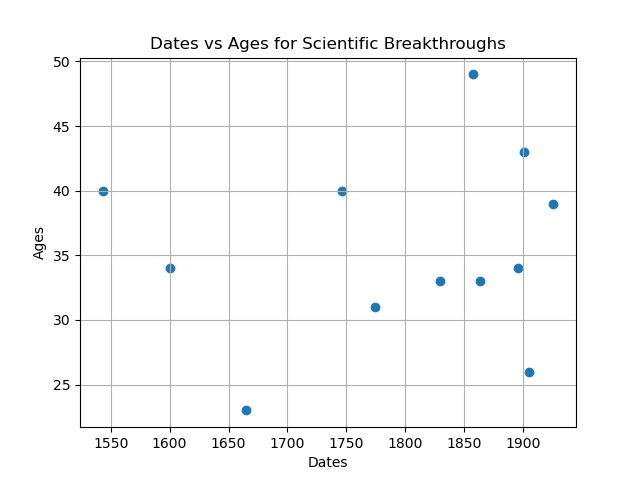
\includegraphics[width=500pt]{science.png}
\end{figure}
\\
\\
The variability in \(y_i\)'s appear to be relatively random with respect to time, with a decent spread over time, although there seem to be slightly more discoveries over time.
\\
\\
The code used is as follows:
\begin{verbatim}
import matplotlib.pyplot as plt

plt.scatter(dates, ages)
plt.xlabel("Dates")
plt.ylabel("Ages")
plt.title("Dates vs Ages for Scientific Breakthroughs")
plt.grid(True)
plt.show()
\end{verbatim}

\section*{7.4.19}

MBAs R Us advertises that its program increases a person's score on the GMAT by an average of forty points. As a way of checking the validity of that claim, a consumer watchdog group hired fifteen students to take both the review course and the GMAT. Prior to starting the course, the fifteen students were given a diagnostic test that predicted how well they would do on the GMAT in the absence of any special training. The following table gives each student's actual GMAT score minus his or her predicted score. Set up and carry out an appropriate hypothesis test. Use the 0.05 level of significance.
\\
\\ 
We set the null hypothesis to be that the program score increase has an average of 40 points, and the alternative hypothesis to be that the program score increase does not have an average of 40 points, i.e. \(H_0: \mu = 40, H_1: \mu \neq 40\).  So this is a two-tailed test. Using the data points and a programming language, we take the respective sums of \(\sum_{i=1}^{15} y_i = 556 \) and \(\sum_{i=1}^{15} y_i^2 = 20966\), as well as the simple arithmetic mean of the sample \(\mu_i = 37.06666666666667\). We can thus take 
\[
s^2 = \frac{ n(\sum_{i=1}^{15} y_i^2) - (\sum_{i=1}^{n} y_i)^2}{n(n-1)}
\]
\[
s^2 = \frac{15 \cdot 20966 - (556)^2}{15 \cdot 14}
\]
\[
s^2 = \frac{314490 - 309136}{210} = \frac{5354}{210} = 25.4952380952
\]
\[
s = 5.04928094833
\]
as the sample standard deviation. We can then do a two tailed t-test to find
\[
t = \frac{\bar{x}-\mu_0}{s/\sqrt{n}}
\]
\[
t = \frac{37.06666666666667 - 40}{5.04928094833 / \sqrt{15}}
\]
\[
t = \frac{-2.93333333333}{1.30371873488} = -2.24997405871
\]
Comparing this with the critical values  at a table for the corresponding z value, with \(df = n - 1 = 15 - 1 = 14\) and \(\alpha = 0.05\). We therefore need to find at \(t_{\alpha / 2, df } = t_{0.05 / 2, 14} = t_{0.025, 14} = -2.1447866879169277 \). The absolute value of this critical value is lower than the absolute value of the test statistic, so we reject the null hypothesis \(H_0\) that the program increases a person's score by an average of forty points. We can find the corresponding p-value to be \(0.04105590880691748\).
\\
\\
The code used is as follows:
\begin{verbatim}
import numpy as np
from scipy import stats

gmat_y_i = [35, 37, 33, 34, 38, 40, 35, 36, 38, 33, 28, 34, 47, 42, 46]
gmat_y_i_squared = [1225, 1369, 1089, 1156, 1444, 1600, 1225,  1296, 1444, 1089, 784, 1156, 2209, 1764, 2116]

gmat_y_i_sum = np.sum(gmat_y_i)
gmat_y_i_squared_sum = np.sum(gmat_y_i_squared)

print(f"{gmat_y_i_sum=}")
print(f"{gmat_y_i_squared_sum=}")

gmat_y_i_mean = np.mean(gmat_y_i)
gmat_y_i_std = np.std(gmat_y_i, ddof = 1)

print(f"{gmat_y_i_mean=}")
print(f"{gmat_y_i_std=}")

gmat_t_value = stats.t.ppf(0.05 / 2, 14)

print(f"{gmat_t_value=}")

gmat_p_value = 2 * stats.t.sf(abs(-2.24997405871), df=14)

print(f"{gmat_p_value=}")
\end{verbatim}
with output:
\begin{verbatim}
~/Doc/e/j/S/Problem Sets/EN.625.603.84/Problem Set 6 problem-set-5 ?1 ............................................. py base 23:13:50
> python gmat_7419.py
gmat_y_i_sum=np.int64(556)
gmat_y_i_squared_sum=np.int64(20966)
gmat_y_i_mean=np.float64(37.06666666666667)
gmat_y_i_std=np.float64(5.049280948336911)
gmat_t_value=np.float64(-2.1447866879169277)
gmat_p_value=np.float64(0.04105590880691748)
\end{verbatim}

\section*{7.5.13}

If a 90\% confidence interval for \(\sigma^2\) is reported to be (51.47, 261.90), what is the value of the sample standard deviation?
\\
\\
We know by definition that a \(100(1 - \alpha) \%\) confidence interval for \(\sigma^2\) is the set of values 
\[
\big(\frac{(n-1)s^2}{\chi^2_{\alpha / 2, n-1}}, \frac{(n-1)s^2}{\chi^2_{1 - \alpha / 2, n-1}}\big)
\]
and we want to find \(s\), so let's solve accordingly. We have the values for these respective values, so we can solve this as a system of equations:

\begin{equation*}
\begin{cases}
51.47 = \frac{(n-1)s^2}{\chi^2_{\alpha / 2, n-1}} \\
261.90 = \frac{(n-1)s^2}{\chi^2_{1 - \alpha / 2, n-1}}
\end{cases}
\end{equation*}

\begin{equation*}
\begin{cases}
51.47 \cdot \chi^2_{\alpha / 2, n-1} = (n-1)s^2 \\
261.90 \cdot \chi^2_{1 - \alpha / 2, n-1} = (n-1)s^2
\end{cases}
\end{equation*}

\begin{equation*}
\begin{cases}
51.47 \cdot \chi^2_{\alpha / 2, n-1} = (n-1)s^2 \\
261.90 \cdot \chi^2_{1 - \alpha / 2, n-1} = (n-1)s^2
\end{cases}
\end{equation*}
Let's solve first for \(n\), knowing that \(\alpha = \frac{-10}{-100} = 0.1\):
\[
51.47 \cdot \chi^2_{\alpha / 2, n-1} = 261.90 \cdot \chi^2_{1 - \alpha / 2, n-1}
\]
\[
51.47 \cdot \chi^2_{0.05, n-1} = 261.90 \cdot \chi^2_{0.95, n-1}
\]
\[
\frac{\chi^2_{0.05, n-1}}{\chi^2_{0.95, n-1}} = \frac{261.90}{51.47} = 5.0884010103
\]
We begin trial and error for \(n\). We test for degrees of freedom \(n-1\):
\[
n = 6, df = 5: \frac{\chi^2_{0.05, 5}}{\chi^2_{0.95, 5}} = \frac{11.070}{1.145} = 9.66812227074
\]
Too high, let's continue:
\[
n = 11, df = 10: \frac{\chi^2_{0.05, 10}}{\chi^2_{0.95, 10}} = \frac{18.307}{3.940} = 4.64644670051
\]
Too low, but close, let's backtrack:
\[
n = 10, df = 9: \frac{\chi^2_{0.05, 9}}{\chi^2_{0.95, 9}} = \frac{16.919}{3.325} = 5.08842105263
\]
This is incredibly close and serves as a viable \(n\), let's continue to find \(s^2\):
\[
51.47 \cdot \chi^2_{0.1 / 2, 10 - 1} = (10 - 1)s^2
\]
\[
51.47 \cdot \chi^2_{0.05, 9} = 9s^2
\]
\[
\frac{51.47 \cdot 16.919}{9} = s^2
\]
\[
s^2 = 96.7578811111
\]
We are looking for \(s\), so we take the square root:
\[
s = 9.83655839769
\]

\section*{7.5.16}

When working properly, the amounts of cement
that a filling machine puts into 25-kg bags have a standard deviation (\(\sigma\)) of 1.0 kg. In the next column are the weights recorded for thirty bags selected at random from a day's production. Test \(H_0: \sigma^2 = 1 \) versus \(H_1: \sigma^2 > 1\) using the \(\alpha = 0.05\) level of significance. Assume that the weights are normally distributed.
\\
\\
To perform this test, we essentially want to take the test statistic \(\chi^2\) and reject the null hypothesis if \(\chi^2 \geq \chi^2_{1-\alpha, n-1}\). 
\\
We take the sample variance \(s^2 = \frac{n \cdot \sum_{i=1}^{n} y_i^2 - (\sum_{i=1}^{n}y_i)^2}{n \cdot (n-1)}\), substituting for the values given in the problem gives us 
\[
s^2 = \frac{30 \cdot 19,195.7938 - 758.62^2}{30 \cdot 29} = \frac{575873.814 - 575504.3044}{30 \cdot 29} = \frac{369.5096}{870} = 0.42472367816
\]
We then take \(\chi^2\) like so:
\[
\chi^2 = \frac{(n-1)s^2}{\sigma_0^2} = \frac{29 \cdot 0.42472367816}{1} = 12.3169866666
\]
We then need to find \(\chi^2_{1-\alpha, n-1} = \chi^2_{0.95, 29} \), looking at a table for the appropriate values gives us 42.557. Our \(\chi^2\) is clearly lower than this, so we fail to reject \(H_0\). In other words, there is not enough evidence to determine at the requisite significance level that the distribution variance is greater than 1.

% End of the large subsection
}

\end{document}